\newpage
\section{Multiples Access and Modulation \formelbuch{51}}
\subsection{Kanalzugriff}
	Den Kanalzugriff muss nur für Systeme mit mehreren unterschidlichen Sender bzw.
	Empfängern geregelt werden. Folgende Möglichkeiten bestehen:\\

\subsubsection{FDMA - Frequency Division Multiple Access - Frequenz-Multiplexing
\formelbuch{52}} Prinzip:\\Jeder Benutzer sendet auf einer zugewiesenen Frequenz mit einer
		definierten Bandbreite.\\
		Einsatzort:\\FM, aber auch GSM im Up-, wie auch im Downlink-Band (siehe
		Bild)\\
\subsubsection{TDMA - Time Division Multiple Access - Zeit-Multiplexing
\formelbuch{52}}

\begin{tabular}{ll}
\parbox{11cm}{
		Prinzip:\\Jeder Benutzer bekommt einen bestimmten Zeitschlitz, um in
		diesem Pakete senden zu können. Nach einer gewissen Zeit (Frame) wiederholt sich das
		ganze\\
		Einsatzort:\\zB. GSM: In einem Frame von 4.615ms hat es jeweils 8
		Teilnehmern (siehe Bild).}
    & \parbox{9cm}{
        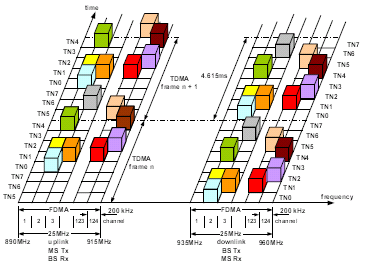
\includegraphics[width=6cm]{./bilder/modulation_TDMA.png}
        } \\
\parbox{11cm}{
		Speziell: ALOHA\\
		Für die Zuordnung der Zeitschlitze für einen neuen Teilnehmer meldet sich
		dieser zuerst bei der Basisstation. Dabei kann es zu Kollisionen mit anderen
		Teilnehmern kommen. Erneutes Melden bei der Basisstation erfolgt beim
		ALOHA-Prinzip nach einer zufällige Zeitdauer, womit die erneute
		Kollision vermieden wird.} 
	& \parbox{9cm}{
	    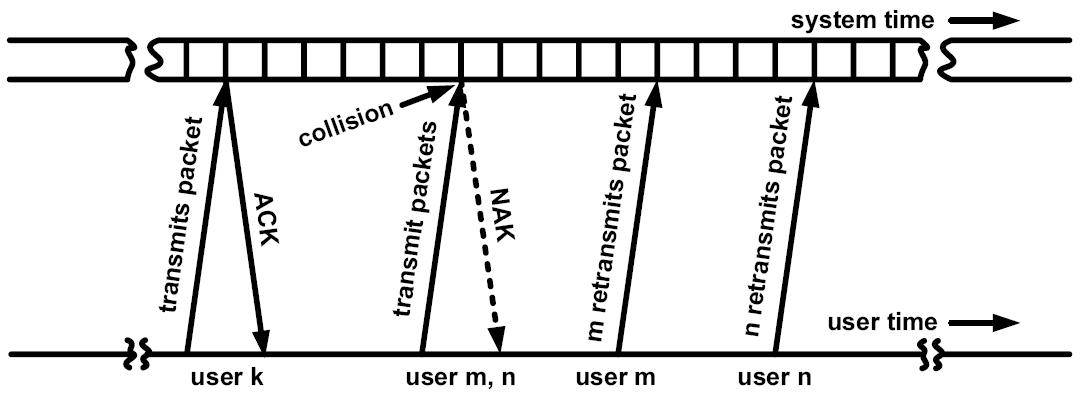
\includegraphics[width=6cm]{./bilder/modulation_aloha.png}
	    }
\end{tabular}

\subsubsection{CDMA - Code Division Multiple Access - Code Multiplexing} 
Prinzip:\\
Die Trägerfrequenzen werden mit Hilfe eines Codes zeitlich variiert. Durch eine
Korrelation mit demselben Codes kann man die richtigen Daten auch bei
Überlagerungen wieder herausfiltern. Deshalb können viele Sender bzw. Empfänger
auf demselben Frequenzband arbeiten. CDMA brauch jedoch durch das
Frequenzhopping auch mehr Bandbreite.\\
Vorteil/Nachteile:\\
+ Die Daten sind nur für die Empfänger mit den richtigen Codes sichtbar.\\
+ Sicher gegen Frequenzlöcher (da CDMA eine grosse Bandbreite benutzt).\\
+ Störsicher gegen schmalbandige Störsignale. \\
+ Bei wenigen Teilnehmern sehr gute SNR\\
+ Gut für unkoordinierte Teilnehmer (da keine Absprachen bezüglich
Zeitschlitz, Kanalfrequenz, etc. nötig sind)\\
- Schlechtes Near-Far-Verhalten
(wenn ein starker (naher) Teilnehmer einen schwachen (fernen) unterdrückt). \\
	
\textbf{Beispiel:} \\
In einem CDMA-System spreizen $K=2$ Benutzer ihre bipolaren Daten-Bits $d_k \in \{-1,+1\}$ 
synchron mit den folgenden Codes mit je $N=7$ Chips: \\
$s_1=[ -1, 1, 1, -1, -1, -1, 1 ]$, 
$s_2=[ -1, 1, 1, -1, 1, -1, -1 ]$, 
$s_3=[ 1, 1, 1, 1, -1, 1, -1 ]$, 
$s_4=[ -1, 1, -1, -1, 1, 1, -1 ]$

Der Empfänger erhält die folgende verrauschte, abgetastete Summen-Chip-Folge \\
$r=[-2, 0, -2, -2, 2, 0, -2]$ 

Um das bipolare Daten-Bit $d_1$ des Benutzer 1 zu bestimmen, kann man folgende
Formel verwenden: \\
$d_1 = sign(r\cdot s_1^T) = sign([-2, 0, -2, -2, 2, 0, -2]\cdot [ -1, 1, 1, -1, -1, -1, 1 ]^T)=sign(-2)=-1$


\subsubsection{OFDM - Orthogonal Frequency Division Multiplexing
\formelbuch{55}}

\begin{tabular}{ll}
\parbox{12cm}{
Funktioniert ähnlich wie FDMA, nur werden hier zueinander orthogonal stehende
Trägersignale verwendet, wobei jeder Träger ein Symbol (ein oder mehrere Bits)
repräsentiert. Laut Definition ist dann: \\
$  \int_0^{T_S} \sin (2\pi f_i t)\sin (2\pi f_j t) dt = 
  \left\{\begin{array}{l@{\,\,\,\,} l}
         0 , &   i\not = j, \\ 
         1 , &   i = j .   \end{array} \right.$\\
Daraus folgt, dass die bei FDMA übliche Sicherheitsabstände zwischen den Trägern
null sind. 
       } 
&
\parbox{6cm}{
    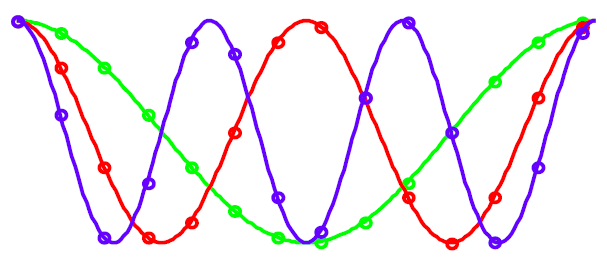
\includegraphics[width=6cm]{./bilder/modulation_OFDM-orthogonal.png}\\
    \small Orthogonalität der Träger
}       
\end{tabular}
\begin{center}
    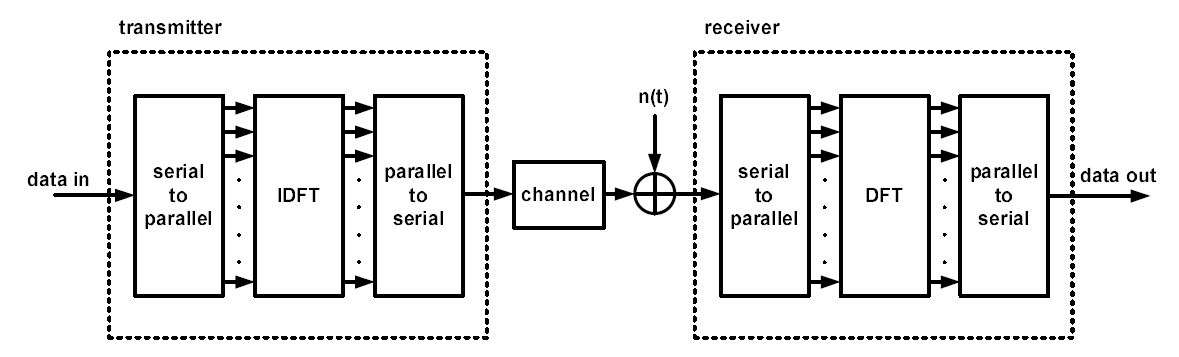
\includegraphics[width=15cm]{./bilder/modulation_OFDM-schematic.png}\\
    \small Blockschaltbild - OFDM Sender und Empfänger
\end{center}

\begin{tabular}{lll}
\parbox{4cm}{
$$\frac W{B_{\text{coh}}} \ll N_c \ll WT_{\text{coh}} $$ 
$$ T_{\text{coh}} < \dfrac{N_c}{R} = T_{\text{Subcarrier}} $$
       } 
&
\parbox{5cm}{
   $W$: Gesamtbandbreite \\
   $\dfrac{W}{N_C}$: Subcarrier Bandbreite \\
   $R$: Symbolrate (gesamtes Band)
}       
&
\parbox{9cm}{
   $N_C$: Anzahl Subcarrier bzw. Kanäle \\
   $B_{\text{coh}}$: Kohärenzbandbreite \\
   $T_{\text{coh}}$: Kohärenzzeit (Zeitinvarianz Übertragungskanal)
}       
\end{tabular}

Im Vergleich zur seriellen Übertragung ergibt sich bei der gleichen
Übertragungsrat eine viel längere Symbolzeit, da die Daten parallel übertragen werden. Dies
ermöglicht es gegenüber Einträgerverfahren, viel weniger Bandbreite zu nutzen.
\\

Problem der \textbf{Multidimensional Interference (MDI)}:
\begin{liste}
    \item \textbf{Intersymbolic Interference (ISI)} \\
            Symbole überlappen sich im Zeitbereich (wegen Faltung mit Impulsantwort des Kanals - Laufzeit, Echo, usw.). 
			Um dies zu vermeiden wird in der Regel ein Guard Intervall $T_{Guard}$ zwischen den Symbolen eingefügt. 
			Wenn ein ISI verhindert werden soll, dann darf der Unterschied zwischen dem LOS-Ausbreitungspfad und einem 
			Nicht-LOS-Ausbreitungspfad maximal $D_{max} = c\cdot T_{Guard}$ sein.
    \item \textbf{Inter Channel Interference (ICI)} \\
            Subcarrier sind nicht mehr orthogonal. \\
\end{liste}

\begin{tabular}{lll}
	\parbox{6cm}{ 
    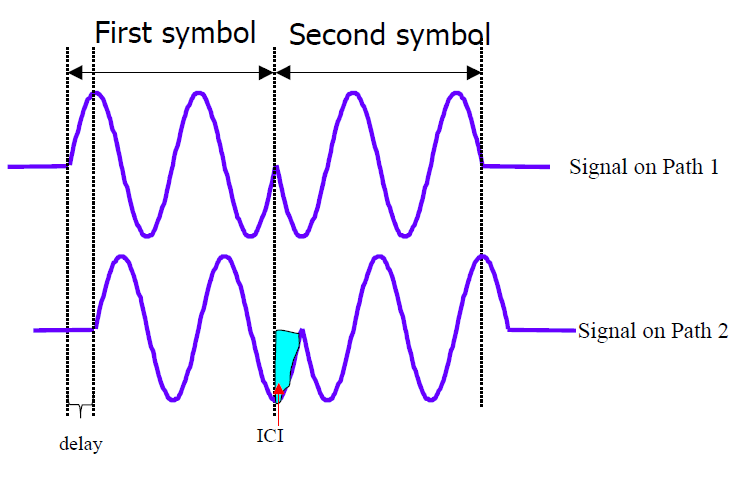
\includegraphics[width=6cm]{./bilder/modulation_OFDM-ICI.png}\\
	}    
	& \parbox{6cm}{Ein nicht-sinusförmiges Signal (Bild links) hätte mehrere/höhere
	Frequenzkomponenten zur Folge, welche in andere Subcarrier überlappen würden -
	\textbf{ICI}. Um dies zu verhindern wird das Signal mit einem sogenannten \textbf{Cyclic
	Prefix} (Bild rechts) versehen, sodass ein reines sinusförmiges Signal
	resultiert. \\	
	} &
	\parbox{6cm}{
	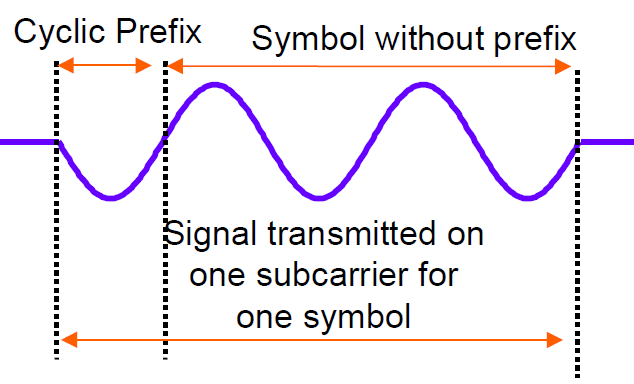
\includegraphics[width=6cm]{./bilder/modulation_OFDM-prefix.png}\\ }       
\end{tabular}


\subsection{Modulation}
Die analogen continuierlichen Modulationsarten wie AM, FM und PM werden hier
nicht behandelt. Es wird von digitalen Daten ausgegangen.

\subsubsection{Komplexes Basisband \formelbuch{57}}
Generell ist ein RF- Signal symmetrisch bezüglich des Nullpunktes
($A_1=A_{-1}$)nicht jedoch bezüglich des RF Trägers. Dies hat zur Folge, dass
das demodulierte Signal nicht mehr symetrisch zu Null ist, was bedeutet, dass
es ein komplexes Spektrum ist. $s_{RF}(t)=\Re(s_{bb}(t)e^{j2\pi f_{RF}t})$\\
\begin{tabular}{lll}
	\parbox{5cm}{
		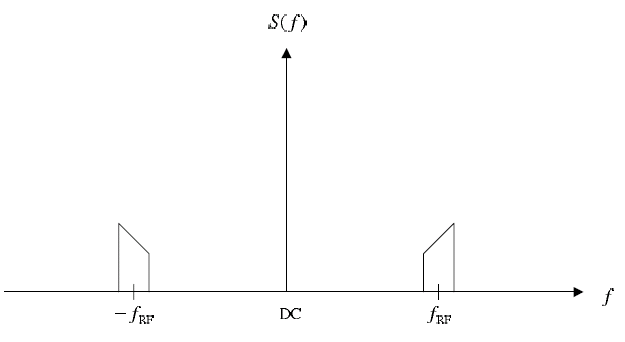
\includegraphics[width=5cm]{./bilder/modulation_RFSpektrum.png}
	}
	&$\Longrightarrow$
	&\parbox{5cm}{
		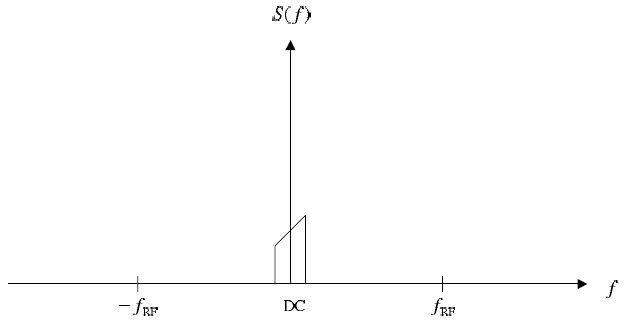
\includegraphics[width=5cm]{./bilder/modulation_BBSpektrum.png}
	}
\end{tabular}

\subsubsection{BPSK - Binary Phase Shift Keying  \formelbuch{58}}
\begin{tabular}{ll}
	\parbox{10cm}{
		\begin{tabular}{ll}
			BPSK&= 2-PAM \\
			Phase $\in \{-180^o, 0$\} &= Amplitude $\in \{-1, 1\}$
		\end{tabular}\\
		Bild rechts zeigt Amplitude und Phase des Basisbandes genau zur sampling
		time.\\
	}
	&
	\parbox{5cm}{
		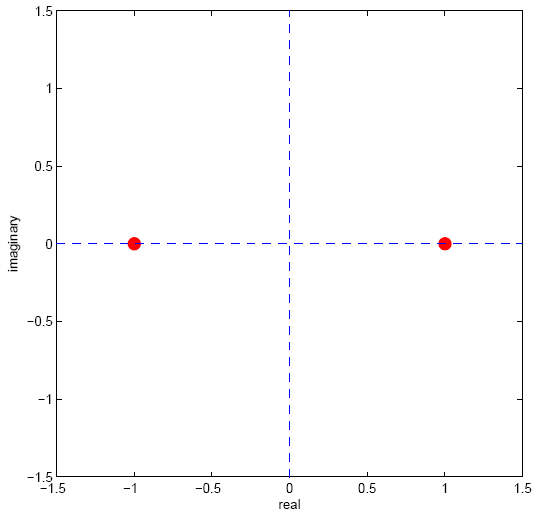
\includegraphics[width=5cm]{./bilder/modulation_constellationBPSK.png}
	}
\end{tabular}
\subsubsection{M-PAM - Pulse Amplitude Modulation \formelbuch{59}}
M kommt von M- Zuständen, welche die Amplitude annehmen kann. Dadurch können
$N=\log_2(M) [\frac{bits}{Symbol}]$ übertragen werden. Durch die Abstufung wird
die Effizienz gesteigert. Da PAM ein reelles Spektrum besitzt ist auch das
RF-Signal symmetrisch zum Träger, was jedoch die Bandbreiteneffizient stark
vermindert. Mögliche Verbesserungen:\\
\begin{liste}
	\item Zusätzlicher Imaginäranteil $\Longrightarrow$ QAM
	\item Grösseres M (Nachteil: grössere Fehlerwahrscheindlichkeit und immernoch
	symetrisch)
	\item Eliminierung des einen Frequenzbandes(z.B mit SSB)
\end{liste}

\subsubsection{M-QAM - Quadratur Amplitude Modluation \formelbuch{61}}
\begin{tabular}{ll}
\parbox{10cm}{
	Bei QAM wird die Phase und Amplidue verändert. Um eine optimale Ausnützung zu
	erhalten soll $M=2^n$ gewählt werden, wobei $n \epsilon \mathbb{N}$ und 
	$n=N=\frac{bit}{Symbol}$ist.\\
	Falls n gerade dann ergibt es ein vollständiges Viereck.\\
	Bei n ungerade ergibt sich ein Viereck ohne die Ecken.\\
	Spezialfall: 4- QAM = QPSK\\
	Das Problem für die MobKom an QAM ist, dass sich die Amplitudedämpfung sehr
	stark und relativ schnell ändern kann. Deshalb kann man keine Information als
	Amplitudenänderung senden, was dann nur noch eine Phasenverschiebung (M-PSK)
	zur Folge hat.} 
	& \parbox{8cm}{
	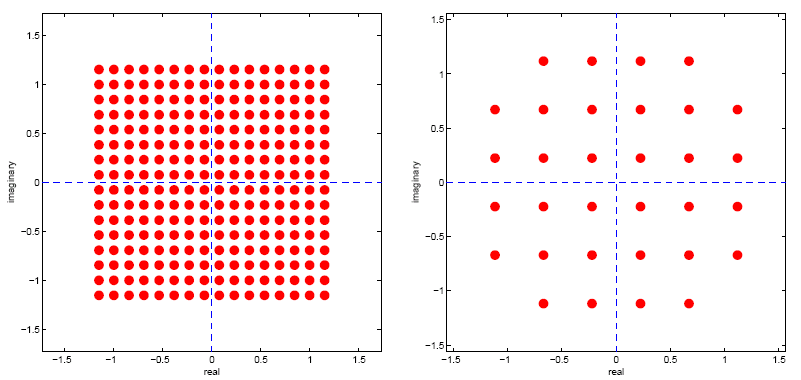
\includegraphics[width=8cm]{./bilder/modulation_constellationQAM.png}\\ 256-QAM und 32-QAM
}
\end{tabular}

\subsubsection{M-PSK - Phase Shift Keying \formelbuch{63}}
\begin{tabular}{ll}
\parbox{10cm}{
Spezielle Formen:\\
\begin{liste}
 \item Bei \textit{D}PSK kommt es nicht mehr auf die
	absolute Phase an, sondern nur noch auf den Phasensprung von Symbol zu Symbol
	(z.B. je $\frac{\pi}{4}$). So ist keine Referenz zur Nullphase nötig.
 \item \textit{$\frac{3\pi}{8}$} oder \textit{EDGE-Modulationschema} wird bei
 GSM eingesetzt. Der Vorsatz \textit{$\frac{3\pi}{8}$} bedeutet, dass zu
 einem normalen Phasensprung (hier $n \frac{\pi}{4}$ nochmals einen Offset
 von $\frac{\pi}{8}$ hinzu kommt. Dies hat zur Folge, dass die komplexe
 Amplitude nie null wird. (siehe Bild)
\end{liste}


}
&\parbox{6cm}{
    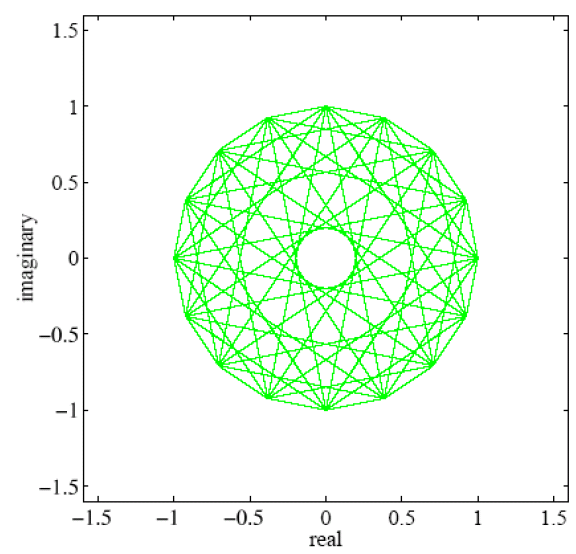
\includegraphics[width=6cm]{./bilder/modulation_constellationEDGE.png}\\
    $\frac{3 \pi}{8}$ 8-PSK

}
\end{tabular}

\subsubsection{Gray- Code \formelbuch{65}}
\begin{tabular}{ll}
	\parbox{8cm}{
		Der Vorteil des Gray Codes gegenüber der normalen binären Codierung ist, dass
		bei einem Fehler nur ein Bit falsch wird und nicht gerade alle, wie das Bild
		rechts zeigt.\\
        Bsp. aus Prüfung (12. März 2007): Vergrösserung des BER, wenn bei QPSK
        die binäre Standardcodierung statt der Gray-Codierung verwendet wird.
        
        Gray: BER = SER/2 \\
        Binär: BER = SER/2 + SER/4 \\
        Verschlechterung: $\Rightarrow 3/2$   \\ \\
        
        Für Gray-Code gilt: $\text{BER} \approx
        \dfrac{\text{SER}}{n_{\text{bits}}}$ } &\parbox{10cm}{
		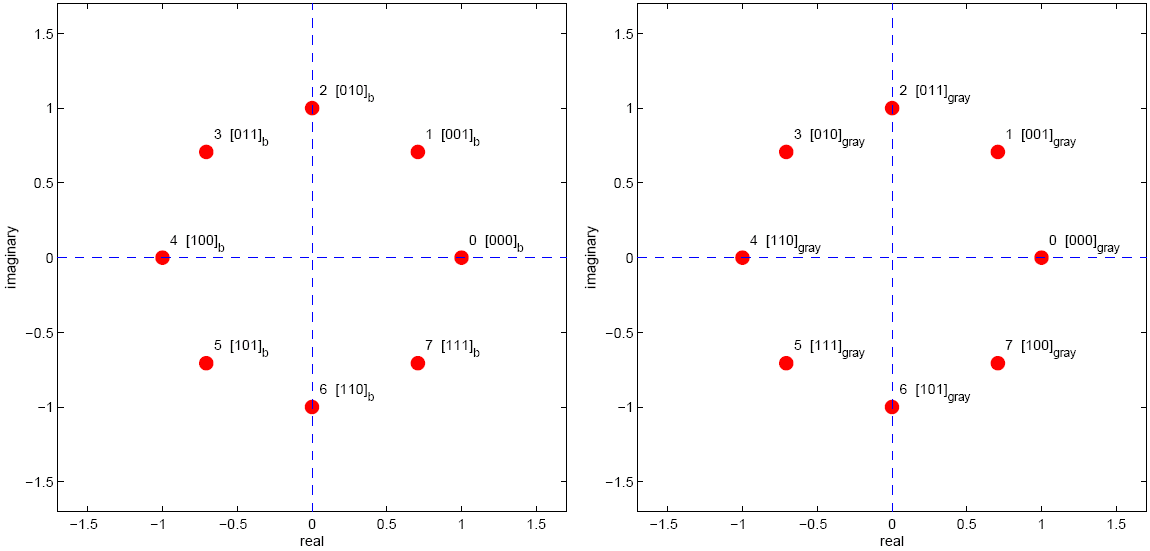
\includegraphics[width=10cm]{./bilder/modulation_PSKmitGray.png}\\
		8-PSK ohne bzw. mit Gray- Code
	}
\end{tabular}

\begin{tabular}{ll}
	\parbox{9cm}{
		\subsubsection{FSK - Frequency Shift Keying \formelbuch{65}}
		Bei FSK wird ein binäres Signal frequenz-moduliert. Das heisst,
		es switscht (hihi) zwischen zwei Frequenzen, dies wird meist mit Hilfe eines
		VCO gemacht.\\
		Kenngrösse ist der Modulations Index: \\
		$h=\dfrac{\Delta f}{f_{\text{data}}}=\dfrac{f_{\text{max}} -
		f_{\text{min}}}{f_{\text{data}}} =\dfrac{n_{\text{T-max}} -
		n_{\text{T-min}}}{n_\text{T}}$ \\ Bei einem \textbf{h von 0.5 }spricht man von
		\textbf{Minimum Shift Keying (MSK)} oder \textbf{Fast} Frequency Shift Keying
		\textbf{(FFSK)}. Trägerfrequenzen können orthogonal sein, solange der
		Modulationsindex das Minimum $h_{\text{min}}$ nicht unterschreitet. \\ $h_{\text{min}} =
		\begin{cases} 1   & \text{unkohärente Detektion} \\                                
                                0.5   & \text{kohärente - phase
                                synchron - Detektion} \end{cases}$\\
        Für unkohärente Detektion sind die beiden Träger orthogonal, wenn gilt:
        \\
        $    \Delta f = \frac{1}{T_{\text{data}}} \cdot n , \qquad n \in \lbrace
        1, 2, 3, \ldots \rbrace $
	}
	&\parbox{9cm}{
	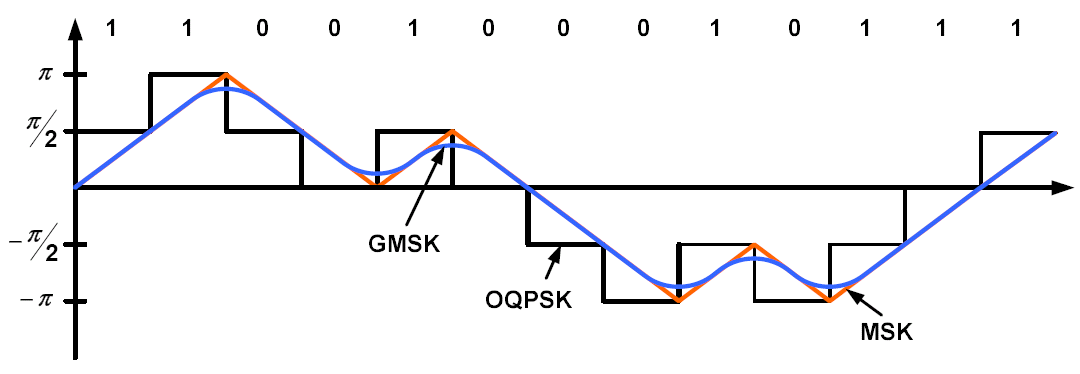
\includegraphics[width=9cm]{./bilder/modulation_phasenverschiebungGMSK_MSK.png}\\
	Phasenverschiebung des MSK bzw GMSK. }
\end{tabular}
     
        
\subsubsection{GMSK - Gaussian Minimum Shift Keying \formelbuch{67}}
Das GMSK ist ein MSK mit einem gauss'schen premodularen Filter, welches eine gauss'sche Pulsform
anstelle der sinusförmigen Pulsform erzeugt. Es besitzt eine
konstante Amplitude und eine grosse spektrale Effizient. 

Bei GSM wurde zu Beginn GMSK verwendet. Siehe Kapitel \ref{sec:gsm} - Modulation.
        

\subsubsection{OQPSK - Offset Quadratur Phase Shift Keying \formelbuch{75, 68}}
Das OQPSK ist eine Sonderform der Quadraturphasenmodulation
	
	
\subsection{Modulationskriterien}
Es gibt 3 Wege um die Fehlerwahrscheinlichkeit
herauszufinden:
\begin{liste}
	\item Austesten und messen (dauert bei kleiner Fehlerwahrscheinlichkeit so
	lange, bis ein vernünftiges Resultat erreicht wird).
	\item Simulieren (dazu ist ein gutes Model nötig, kann unter Umständen gleich
	lange dauern wie austesten).
	\item Analystisch mit Symbol- und Biterrorrate.
\end{liste}
\subsubsection{SER - Symbolfehlerrate \formelbuch{70}}
\begin{tabular}{ll}
\parbox{8cm}{
    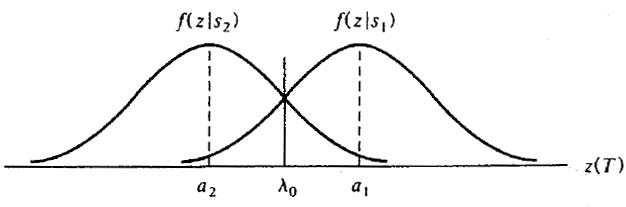
\includegraphics[width=8cm]{./bilder/modulation_AWGN.jpg}
    }
& \parbox{9cm}{
	Die Symbolfehlerrate wird unter anderem verursacht durch das thermische
	Rauschen (AWGN). Dieses hat die Energie\\ 
	$\sigma^2=\frac{N_0}{2}$ \\
	\\
	Die Fehlerwahrscheinlichkeit ist $P_E=Q(\sqrt{\frac{2 E_S}{N_0}})$ mit $a_1 =
	E_S, a_2 = -E_S$ und $\lambda_0 = 0$\\
    }
\end{tabular}

\small
\renewcommand{\arraystretch}{0.6}
% \hspace*{10mm}
\begin{tabular}[ht]{|l|l|l|l|l|}\hline
Modulation & levels/ & normalized & SER (AWGN)
           & Comments \\
scheme     & range   & amplitude  &     &          \\
\hline \hline
%&&&&\\[-3mm]
BPSK & $\pm A$& $A=1$ &
  $Q{(\sqrt{\frac{2E_s}{N_0}})}$ & \\[2mm]  \hline
%&&&&\\[-3mm]
DPSK & $\pm A$& $A=1$ &
  $2Q(\sqrt{\frac{2E_s}{N_0}})$ & coherent \\ 
  &&& $\frac{1}{2}e^{-\frac{E_s}{N_0}}$ & noncoherent\\[2mm] 
\hline
%&&&&\\[-3mm]
QPSK & $(\pm 1\pm j)A$ & $A=\frac{1}{\sqrt{2}}$&
  $ 1-\left(1-Q(\sqrt{\frac{E_s}{N_0}})\right)^2$ & coherent \\[2mm] \hline
%&&&&\\[-3mm]
DQPSK &$(\pm 1\pm j)A$ & $A=\frac{1}{\sqrt{2}}$& 
  $ 2\left(1-\left(1-Q(\sqrt{\frac{E_s}{N_0}})\right)^2\right)$ & coherent \\
&&&  $\frac{1}{2}e^{-\frac{E_s}{2N_0}}$ & noncoherent\\[2mm] \hline
%&&&&\\[-3mm]
$M$-PSK & $ \frac{1}{M}\sum_{m=1}^{M}
             A\delta\left(x- e^{j(2m-1)\frac{\pi}{M}}\right),$ & $A=1$&
  $ \leq 2Q(\sqrt{\frac{2E_s}{N_0})\sin\frac{\pi}{M}})$
  & coherent \\
& $\qquad \qquad \qquad \qquad \,\,\,\,\, m\le M$ &&& \\[2mm] \hline
%&&&&\\[-3mm]
$M$-PAM & $\pm (2m-1)A,\quad m\le M/2$ & $A=\sqrt{\frac{3}{M^2-1}}$ &
  $2\frac{M-1}{M}Q\left(\sqrt{\frac{E_s}{N_0}}\sqrt{\frac{6}{M^2-1}}\right)$ &
  \\[2mm]  \hline
%&&&&\\[-3mm]
$M$-QAM & $(\pm (2m-1)\pm j(2n-1))A,$ & $A=\sqrt{\frac{3}{2(M-1)}}$ 
  &$1-\left(1-2\frac{\sqrt{M}-1}{\sqrt{M}}Q\left(\sqrt{\frac{E_s}{N_0}}
   \sqrt{\frac{3}{M-1}}\right)\right)^2$ & \\
& $\qquad \qquad \quad m,n\le \sqrt{M}/2$ &&& \\[2mm] \hline
%&&&&\\[-3mm]
2-FSK &$\Delta f=h\cdot \frac{1}{T},\, h_{\min}=0.5$ &&
  $Q(\sqrt{\frac{E_s}{N_0}})$ 
  & orthogonal, coherent  \\
& \qquad \qquad \quad $h_{\min}=1$ &&
  $\frac{1}{2}e^{-\frac{E_s}{2N_0}}$ 
  & orthogonal, noncoherent \\[2mm] \hline
\end{tabular}
\renewcommand{\arraystretch}{1}


\subsubsection{BER - Bitfehlerrate \formelbuch{72}}
\begin{tabular}{ll}
	\parbox{10.5cm}{
	Sobald eine Informationsrate R kleiner als die Kanalkapazität C ist, sind
	fehlerfreie Übertragungen möglich.\\
	$C= W \log_2 ( 1+\frac{S}{N}) > R$\\
	Wobei W die Bandbreite des Kanals, N die Rauschenergie $N=N_0 W$ und S die
	Signalenergie ist.
	Die Grenze ist bei $C=R \Longrightarrow E_b C$ $E_b$ ist die Bitenergie\\

	$\Longrightarrow \frac{C}{W}= \log_2(1+\frac{E_b C}{N_0 W})$\\ 

	
	\subsubsection{Spektrale Effizient \formelbuch{75}}
	Heisst wieviel Bandbreite pro Datenrate gebraucht wird.
	Die Effizient beinhaltet zwei Kriterien:
	\begin{enumerate}
	\item Wieviele Bits können in einer gegeben Bandbreite übertragen werden. Wenn
	man die Begrenzung durch die SNR beliebig erweitern indem man die Bits/Symbol
	erhöht.
	\item Wieviel das Spektrum die Nachbarn überlagert. Je nach Modulation gibts
	einen breiten Mainlobe mit schwachen Sidelobes oder umgekehrt.
    \end{enumerate}
  
%    \subsubsection{Raised-Cosine-Filter \formelbuch{63}}
%    $h(t) = \frac{\sin\left((t/T)\pi\right)}{(t/T)\pi}\cdot
%        \frac{\cos\left(\rho(t/T)\pi\right)}{1-4\rho^2(t/T)^2}$\\
%   
%    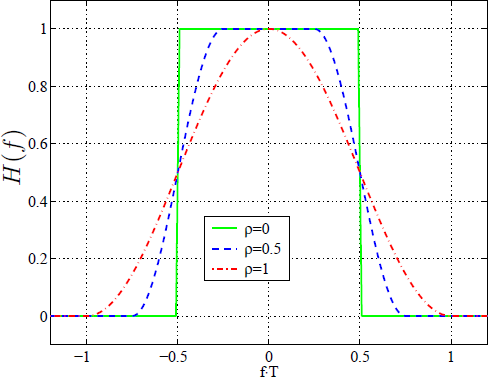
\includegraphics[width=5cm]{./bilder/modulation_raised_cosine_frequency.png}
%    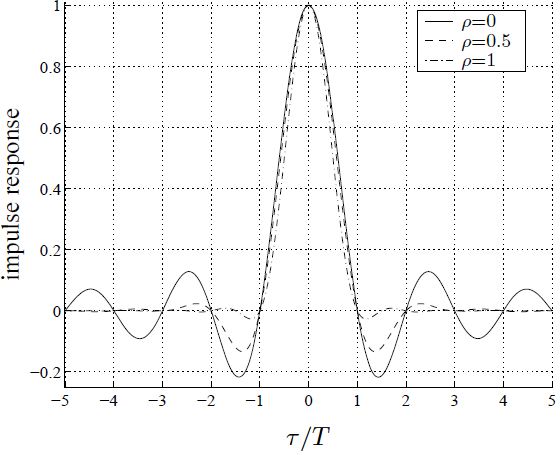
\includegraphics[width=5cm]{./bilder/modulation_raised_cosine_time.png} 
%    
%    Das \textbf{Root-Raised-Cosine-Filter} entspricht der Wurzel des
%    Raised-Cosine-Filters und wird angewendet, wenn die Charakteristik 
%    des Raised-Cosine-Filters auf Sender und Empfänger
%    gleichmässig verteilt werden soll.
    } &\parbox{7cm}{
	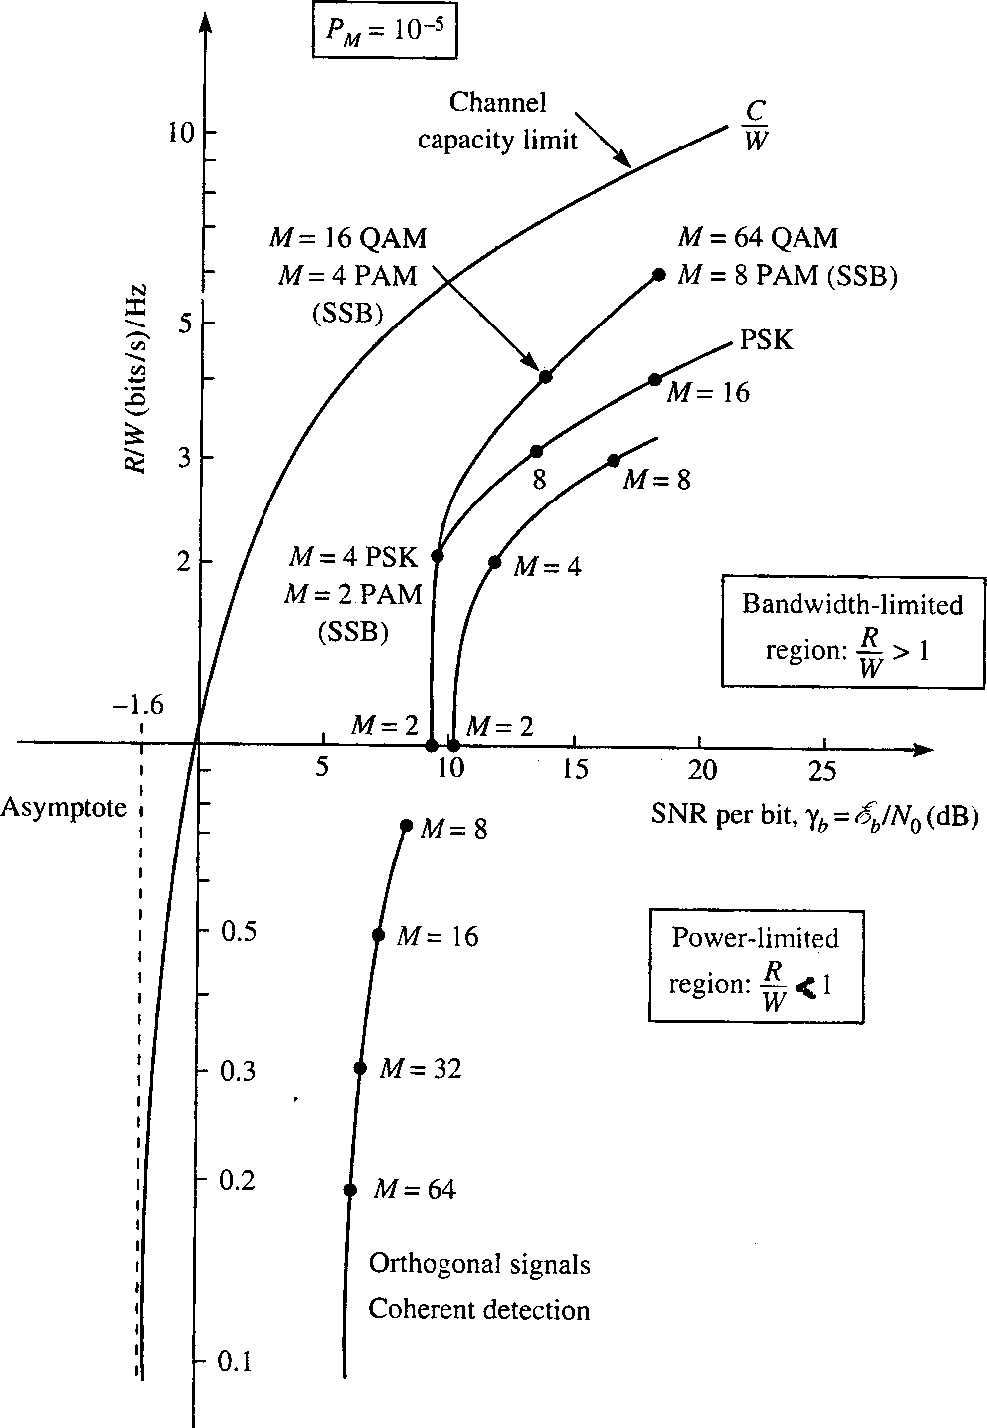
\includegraphics[width=7cm]{./bilder/modulation_SER.png}\\
	Übersicht einzelner Modulationen mit einer SER von $10^{-5}$
	}
\end{tabular}

\subsubsection{Kanalcodierung mit FEC \formelbuch{2-12}}
	\begin{tabular}{ll}
		\parbox{11cm}{
			Mit Interleaving kann eine Verbesserung der BER erreicht werden, vorallem in Bezug auf Fading. 
			Bei diesem Verfahren werden die Büschelfehler (engl. burst errors) durch Verschachtelung 
			auf mehrere Codewörter verteilt, damit die Fehlerkorrektur besser funktioniert.\\
			Im Prinzip werden bei Bit-Interleaving die Codewörter im Zeitmultiplex übertragen.
			Wenn vier Bit hintereinander verfälscht werden, betrifft dies je ein Bit pro Codewort.\\
			\fbox{ 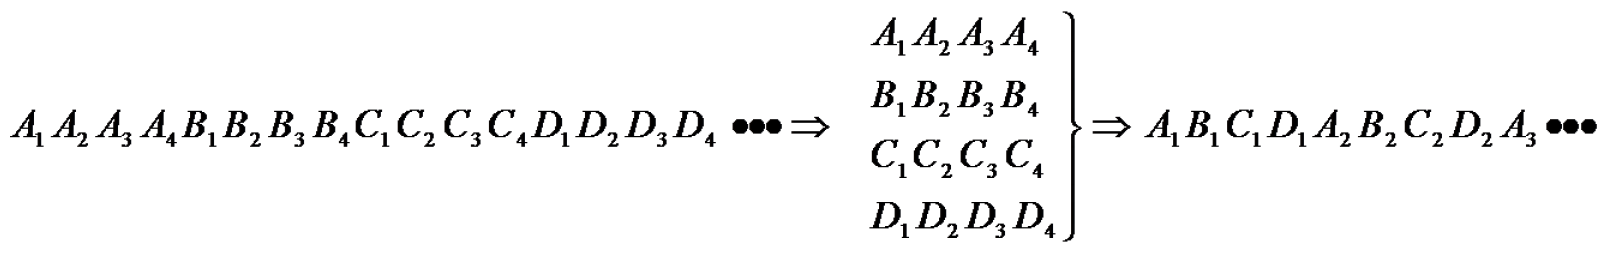
\includegraphics[width=11cm]{./bilder/modulation-interleaving.png}}
		}	
		& \parbox{7cm}{
			\fbox{ 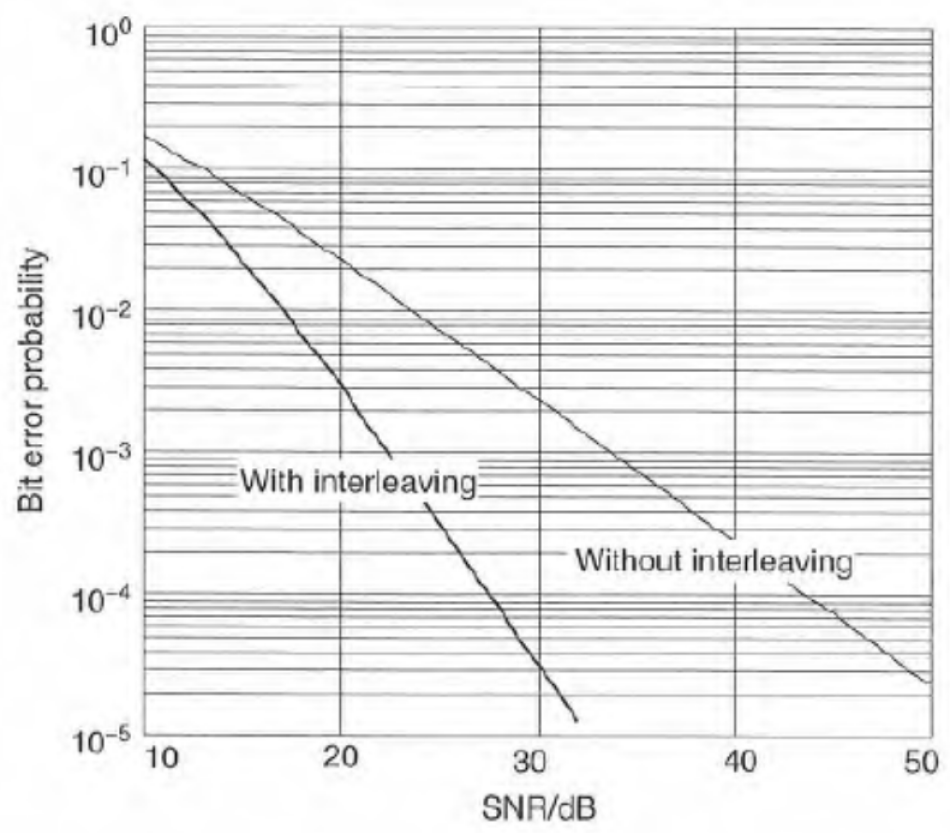
\includegraphics[width=6.5cm]{./bilder/modulation-interleaving-snr.png}}
		}
	\end{tabular}
	
\subsubsection{Faltungscode und Viterbi-Decodierung}
	Als Beispiel eines fehlerkorrigierenden Faltungcodes wird stellvertretend die Viterbi-Codierung erläutert.\\
	\begin{tabular}{ll}
		\parbox{6cm}{
			\fbox{ 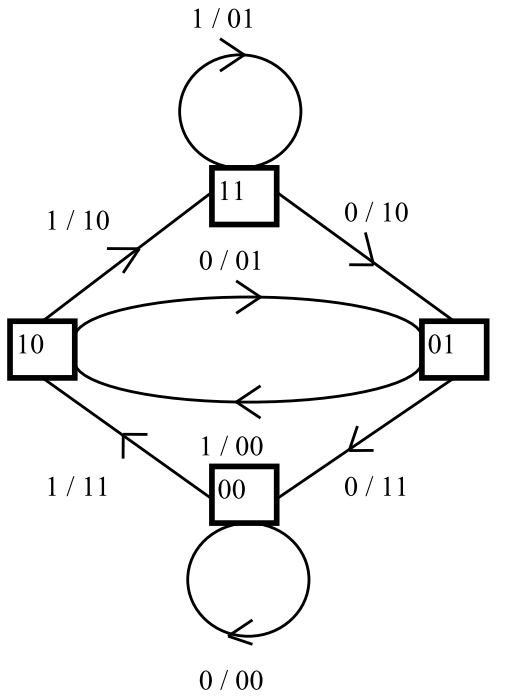
\includegraphics[width=5cm]{./bilder/modulation-viterbi-coder.png}} \\ 
			\textit{Viterbi-Coder:} Man startet immer beim 00-Zustand und hört auch dort wieder auf.
		}	
		& \parbox{12cm}{
			\fbox{ 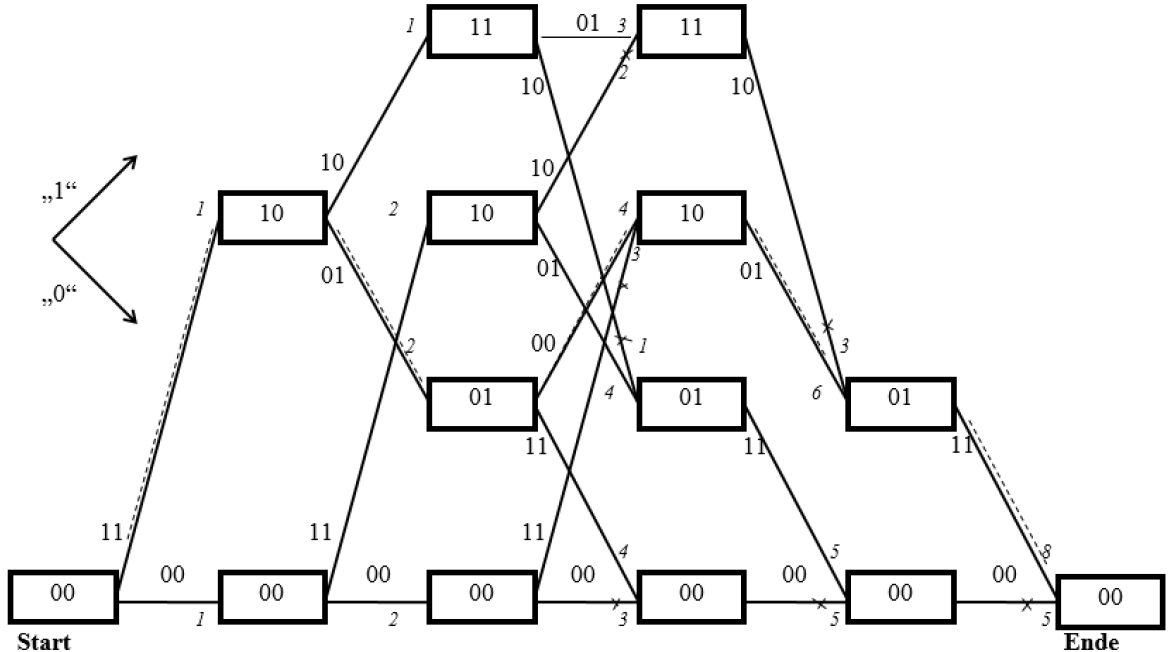
\includegraphics[width=12cm]{./bilder/modulation-viterbi-decoder.png}} \\ 
			\textit{Viterbi-Decoder:} Man geht zuerst von links nach rechts und addiert die übereinstimmenden
			bits des $Y_{empfangen}$ für alle möglichen Pfade. Danach geht man vom Ende zurück und
			wählt den Pfad mit den meisten Punkten. Dies ergibt den $Y_{fehlerkorrigiert}$ und
			daraus kann man die decodierten Daten ermitteln.
		}
	\end{tabular}
	
